%%%%%%%%%%%%%%%%%%%%%%%%%%%%% Define Exam %%%%%%%%%%%%%%%%%%%%%%%%%%%%%%%%%%
\documentclass[addpoints]{exam}
%%%%%%%%%%%%%%%%%%%%%%%%%%%%%%%%%%%%%%%%%%%%%%%%%%%%%%%%%%%%%%%%%%%%%%%%%%%%%%%

%%%%%%%%%%%%%%%%%%%%%%%%%%%%% Using Packages %%%%%%%%%%%%%%%%%%%%%%%%%%%%%%%%%%
\usepackage{amsmath, amssymb, amsthm, amsfonts, geometry, venndiagram}
\usepackage{graphicx, xcolor, color, wrapfig, parskip, float, tabularx}
\usepackage[breaklinks]{hyperref}
\usepackage{colortbl}
\usepackage{listings, mdframed, subfig, matlab-prettifier, hyperref}
\usepackage{lipsum, bookmark, booktabs, empheq, titlesec, verbatim, subfig, pdfpages, comment}
%%%%%%%%%%%%%%%%%%%%%%%%%%%%%%%%%%%%%%%%%%%%%%%%%%%%%%%%%%%%%%%%%%%%%%%%%%%%%%%
\definecolor{codebackground}{rgb}{0.95,0.95,0.95}
\definecolor{codegray}{rgb}{0.5,0.5,0.5}
\definecolor{codepurple}{rgb}{0.58,0,0.82}
\definecolor{codeblue}{rgb}{0.13,0.29,0.53}
\definecolor{ocre}{RGB}{243,102,25}
\definecolor{mygray}{RGB}{243,243,244}
\definecolor{deepGreen}{RGB}{26,111,0}
\definecolor{shallowGreen}{RGB}{235,255,255}
\definecolor{deepBlue}{RGB}{61,124,222}
\definecolor{shallowBlue}{RGB}{235,249,255}
\definecolor{softgray}{rgb}{0.95, 0.95, 0.95}
\definecolor{codegreen}{rgb}{0,0.6,0}
\definecolor{codegray}{rgb}{0.5,0.5,0.5}
\definecolor{codepurple}{rgb}{0.58,0,0.82}
\definecolor{backcolour}{rgb}{0.95,0.95,0.92}

%Code listing style named "mystyle"
\lstdefinestyle{mystyle}{
  backgroundcolor=\color{backcolour}, commentstyle=\color{codegreen},
  keywordstyle=\color{magenta},
  numberstyle=\tiny\color{codegray},
  stringstyle=\color{codepurple},
  basicstyle=\ttfamily\footnotesize,
  breakatwhitespace=false,         
  breaklines=true,                 
  captionpos=b,                    
  keepspaces=true,                 
  numbers=left,                    
  numbersep=5pt,                  
  showspaces=false,                
  showstringspaces=false,
  showtabs=false,                  
  tabsize=2
}

%"mystyle" code listing set
\lstset{style=mystyle}


%%%%%%%%%%%%%%%%%%%%%%%%%%%%% Header and Footer %%%%%%%%%%%%%%%%%%%%%%%%%%%%%%%%%%
\pagestyle{headandfoot}
\runningheadrule
\runningfootrule
\runningheader{Algorithms: Design and Analysis}{Weekly Challenge 01}{CS 412}
\runningfooter{}{Page \thepage\ of \numpages}{}
\firstpageheader{}{}{}
%%%%%%%%%%%%%%%%%%%%%%%%%%%%%%%%%%%%%%%%%%%%%%%%%%%%%%%%%%%%%%%%%%%%%%%%%%%%%%%

% Other Settings
% \boxedpoints
\printanswers
\qformat{}  %Comment this to number questions, uncomment this to not number questions

\newcommand\union\cup
\newcommand\inter\cap

%%%%%%%%%%%%%%%%%%%%%%%%%%%%%%% Title & Author %%%%%%%%%%%%%%%%%%%%%%%%%%%%%%%%

\title{Algorithms: Design and Analysis - CS 412 \vspace*{-4mm}}
\author{Weekly Challenge 01: Getting Started...}
\date{\vspace*{-4mm} Ali Muhammad Asad - aa07190}

% \pgfplotsset{compat=1.18}

%%%%%%%%%%%%%%%%%%%%%%%%%%%%%%%%%%%%%%%%%%%%%%%%%%%%%%%%%%%%%%%%%%%%%%%%%%%%%%%

\begin{document}
\maketitle

% {\small \begin{center} \gradetable[h] \end{center}}

\begin{questions}
  \question[1]
  \textbf{1.}\; (1 point)

  % $ f(n) $ is $ O(g(n)) $ if there exist positive numbers $c$ and $n_0$ such that $ f(n) \leq cg(n) \;\; \forall n \geq n_0  $ \\
  % Let $ f(n) = 2n^2 + 3n + 1 = O(n^2)$. (i) Plot the running time of $ cg(n) $ for different values of $c$ and $n_0$. You may use values for $N (n_0) $ starting with 1, 2, 3, 4, and 5. Plot the function $f(n)$ together with $g(n)$ [with different values of $c$ and $n_0$] with values of $n_0$ on the $X - axis$ and the corresponding values of $f(n)$ and $ cg(n) $ on the $Y - axis$. What is the smallest value of $c$ for which $ f(n) = O(g(n)) $?

  \begin{table}[H]
    \centering
    \resizebox{1.0\textwidth}{!}{
      \begin{tabular}{c c c c c c c c c}
        \rowcolor{lightgray}
        c & $ \geq 6 $ & $ \geq 3\frac{3}{4} $ & $ \geq 3\frac{1}{9} $ & $ \geq 2\frac{13}{16} $ & $ \geq 2\frac{16}{25} $ & $ \cdots $ & $ \to $ & $ 2 $ \\ \hline
        \rowcolor{lightgray}
        $N$ & $ 1 $ & $ 2 $ & $ 3 $ & $ 4 $ & $ 5 $ & $ \cdots $ & $ \to $ & $ \infty $ \\
      \end{tabular}
    }
  \end{table}

  \begin{solution}
    Considering $ g(n) = n^2 $, we get the following plot for varying $c$:
    \begin{figure}[H]
      \centering
      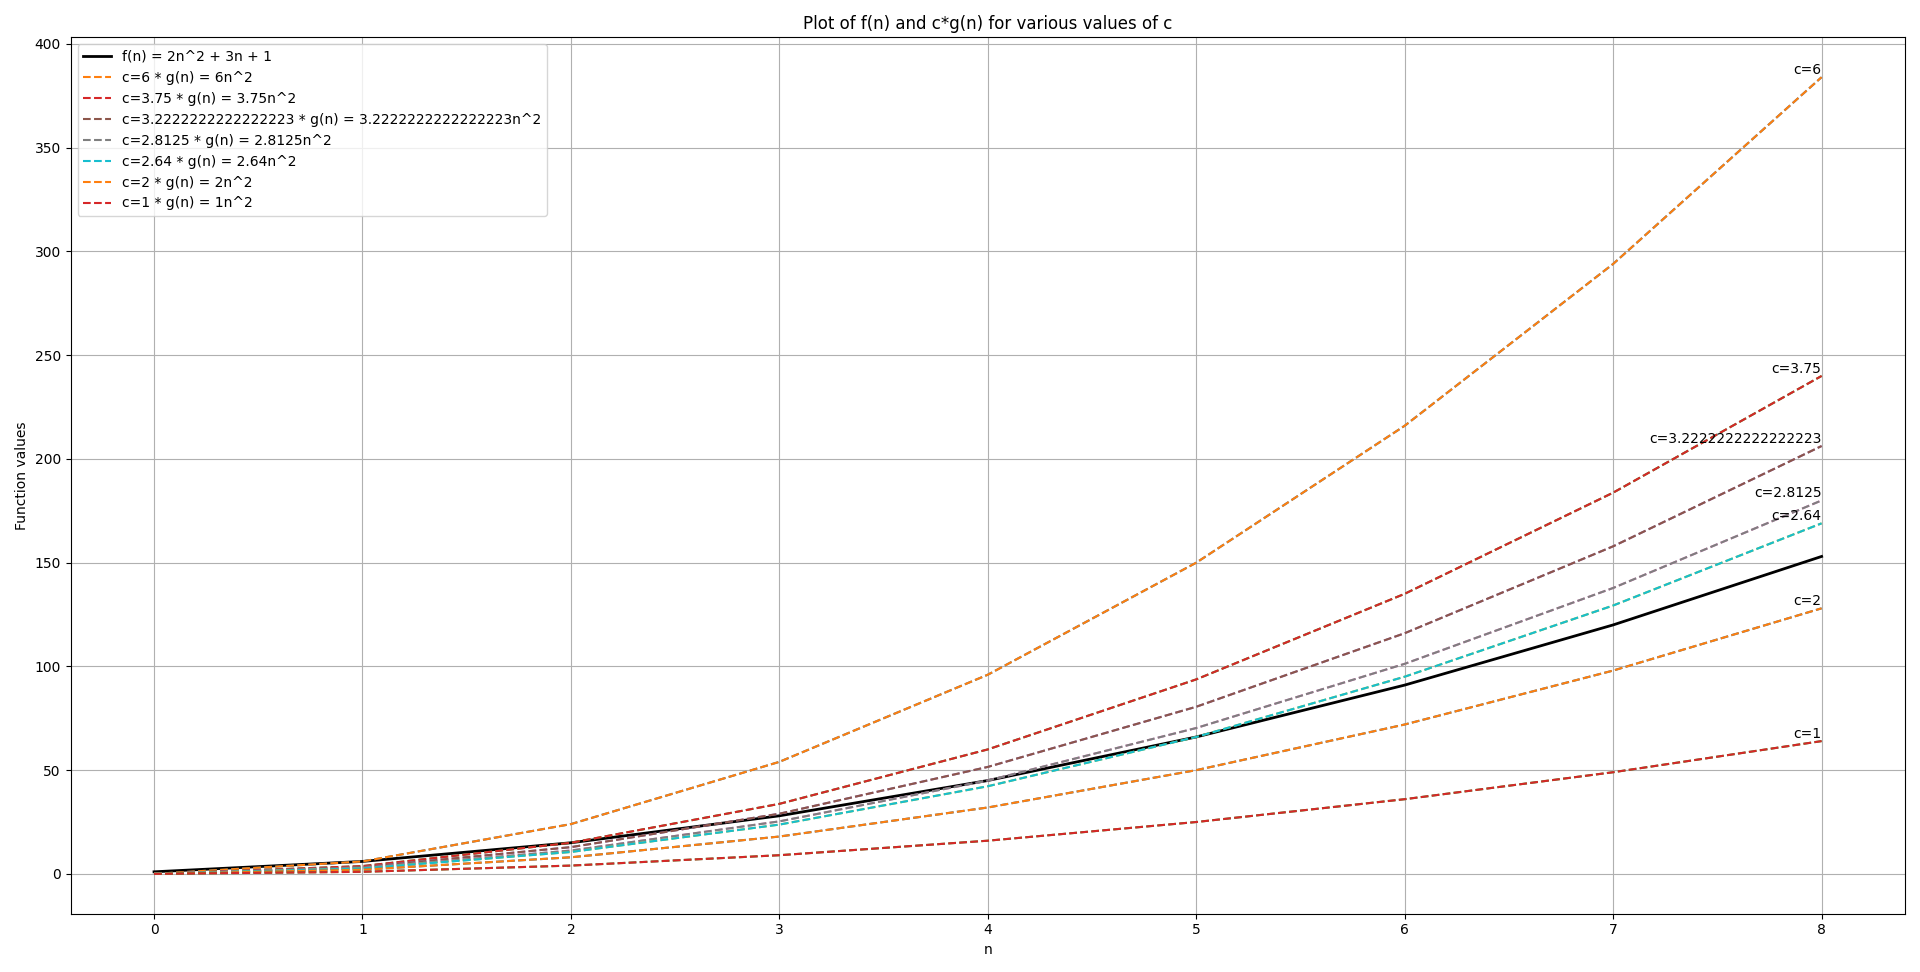
\includegraphics[width=0.95\textwidth]{Figure_1.png}
      \caption{ Plot of $f(n)$ and $cg(n)$ for different values of $c$ and $n_0$ }
    \end{figure}

    Based on the plot shown above, it is clear that as values of $c$ increase, the value of $n_0$ decreases. This is because the function $cg(n)$ increases at a faster rate than $f(n)$, and therefore, the value of $n_0$ decreases as $c$ increases. Then the smallest value of $n_0$ for which $ f(n) = O(g(n)) $ is $ n_0 = 1 $, with $ c = 6 $ as the corresponding $c$ value.

    % This is only based on speculation though from the graph. We can also observe that for $ c = 2 $, $f(n)$ is very close to $cg(n)$, albeit always above since for large values of $n$, $n^2$ becomes the dominating term. 
    % Then $ \exists \varepsilon $ such that $ 2 + \varepsilon $ is the smallest value of $c$ for which $ f(n) = O(g(n)) $. Plugging in values of $ \varepsilon $, we get the following values of $c$ and $n_0$:

    % \begin{center}
    %   \begin{tabular}{c | c | c | c | c}
    %     $ \mathbf{\varepsilon} $ & 0.1 & 0.01 & 0.001 & 0.0001\\ \hline
    %     $\mathbf{c}$ & 2.1 & 2.01 & 2.001 & 2.0001 \\ \hline
    %     $ \mathbf{n_0} $ & 30.3 & 300.3 & 3000.3 & 30000.3 
    %   \end{tabular}
    % \end{center}

    \textit{*Note: The python script for the plot can be found at the end of the pdf}
  \end{solution}

  \newpage
  \question[1]
  \textbf{2.}\; (1 point)

  In computer science, $ lg(n) $ by default refers to $ log $ to the base of 2. The log function appears frequently in asymptotic analysis and often, we ignore the base when performing asymptotic analysis. Does base really matter in asymptotic analysis? Plot the function $ lg(n) $ with bases 2, 7, 10, 100 for `large values' of $n$. Write your observations (in two to three sentences only).

  \begin{solution}
    The below figure shows the plot of differnet bases of the log function:
    \begin{figure}[H]
      \centering
      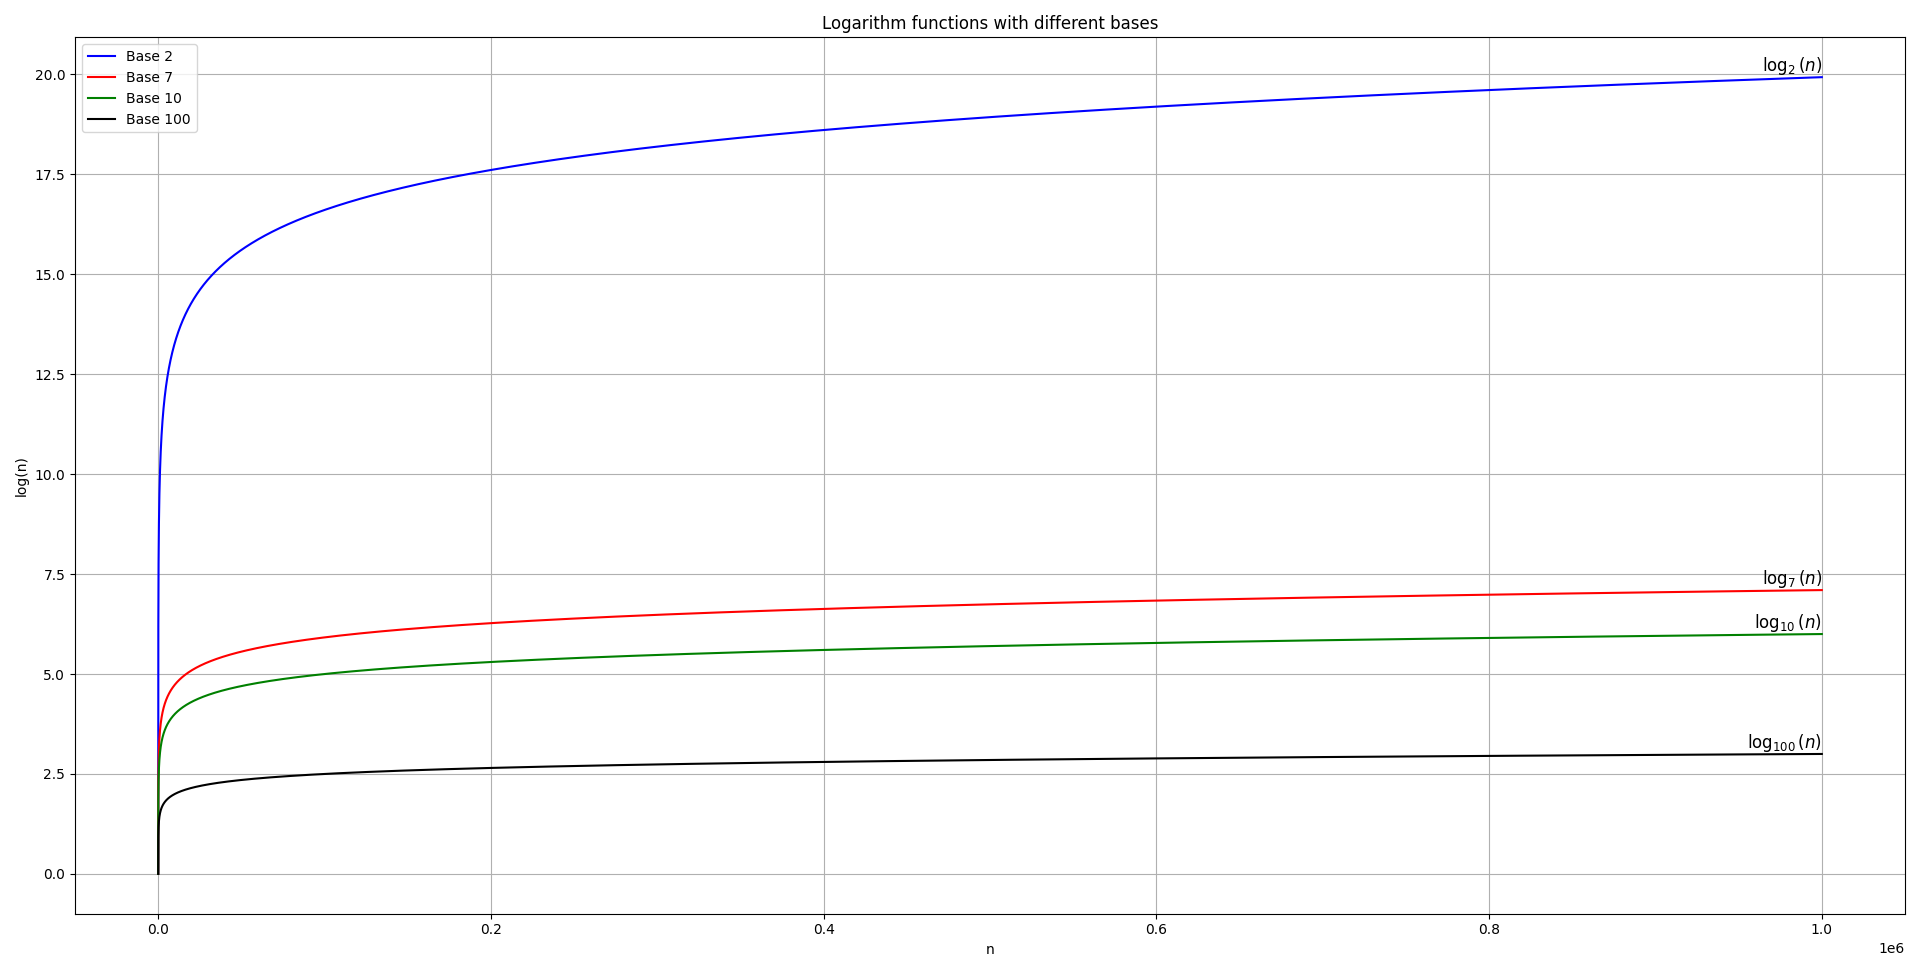
\includegraphics[width=1\textwidth]{Figure_2.png}
      \caption{Plot of different bases of the log function}
    \end{figure}

    Its clear that while the logarithmic functions diverge from each other, they all increase at a decreasing rate and maintain the same overall shape. This indicates that the base of the logarithm affects the scale of the function but not the growth category. In asymptotic analysis, what matters is the growth rate relative to the size of the input; therefore, changing the base of the logarithm only changes the constant factor, which is not considered in Big-O notation. 

    Therefore, the base of the logarithm does not matter in asymptotic analysis, as all logarithms are within a constant factor of each other regardless of the base used. 

    \textit{*Note: The python script for the plot can be found at the end of the pdf}
  \end{solution}
\end{questions}

\newpage
\textbf{Script 1}
\begin{lstlisting}[language=Python, caption=Python script for plotting $f(n)$ and $cg(n)$]
import numpy as np
import matplotlib.pyplot as plt

n = np.arange(0, 9, 1) 

f_n = 2*n**2 + 3*n + 1; g_n = n**2

plt.figure(figsize=(20, 10))

plt.plot(n, f_n, label='f(n) = 2n^2 + 3n + 1', color='black', linewidth = 2)

c_values = [6, 15/4, 29/9, 45/16, 66/25, 2, 1]  # example c values
for c in c_values:
    cg_n = c * g_n
    plt.plot(n, cg_n, linestyle = '--', linewidth = 1.5)
    plt.text(n[-1], cg_n[-1], f'c={c}', ha = 'right' , va = 'bottom')
    plt.plot(n, c*g_n, label=f'c={c} * g(n) = {c}n^2', linestyle='--')

plt.title('Plot of f(n) and c*g(n) for various values of c')
plt.xlabel('n'); plt.ylabel('Function values')
plt.legend(); plt.grid(True)
plt.show()
\end{lstlisting}


\textbf{Script 2}
\begin{lstlisting}[language=Python, caption=Python script for plotting logarithmic functions]
import numpy as np
import matplotlib.pyplot as plt

n = np.arange(1, 1000001)  # Adjust as needed for 'large values' of n

log2_n = np.log2(n)  # Base 2
log7_n = np.log(n) / np.log(7)  # Change of base to 7
log10_n = np.log10(n)  # Base 10
log100_n = np.log(n) / np.log(100)  # Change of base to 100

plt.figure(figsize=(20, 10))

plt.plot(n, log2_n, label='Base 2', color='blue')
plt.plot(n, log7_n, label='Base 7', color='red')
plt.plot(n, log10_n, label='Base 10', color='green')
plt.plot(n, log100_n, label='Base 100', color='black')

plt.title('Logarithm functions with different bases')
plt.xlabel('n'); plt.ylabel('log(n)')
plt.legend(); 
plt.text(n[-1], log2_n[-1], r'$\log_2(n)$', fontsize=12, verticalalignment='bottom', horizontalalignment='right')
plt.text(n[-1], log7_n[-1], r'$\log_7(n)$', fontsize=12, verticalalignment='bottom', horizontalalignment='right')
plt.text(n[-1], log10_n[-1], r'$\log_{10}(n)$', fontsize=12, verticalalignment='bottom', horizontalalignment='right')
plt.text(n[-1], log100_n[-1], r'$\log_{100}(n)$', fontsize=12, verticalalignment='bottom', horizontalalignment='right')
plt.grid(True); plt.show()

\end{lstlisting}

\end{document}